\section{Evaluation}
\label{eg:results}

We test the estimator, the resulting finite designs, and the additional cost
of validation separately. All thermal studies use ideal zero-temperature
exterior and cavity walls. The matched design studies minimize a normalized
regional temperature with a distinct adjoint; the query study additionally
tests distributed-heating compliance, for which $p=u$. Detailed protocols, all comparisons, and step-by-step derivations are
in the appendix. The initial FEM experiment is an independent field check,
not an optimized FEM design-time baseline.

\paragraph{Actual-geometry estimator comparison.}
Eight fixed feasible sites on each of three meshes are evaluated using direct
TWoS, shared-stream finite-cavity subtraction, a stronger stopped-path harmonic
correction, and multigrid with longest-axis grid counts 49, 65, 97, and 129.
The stochastic methods use sixteen repetitions at 256 and 2,048 paths per
site. A separate sixteen-batch, 8,192-path reference estimates the infinitesimal
coefficient; it is not exact ground truth. Trial radii are 0.08, 0.04, 0.02,
and 0.01. The stronger finite-hole baseline estimates the finite correction
from a perforated-domain exit walk and a fresh original-domain state walk
only when the cavity is hit. Its exact harmonic identity and proof appear in
\cref{app:submissionstudy}.

\Cref{eg:submissionestimators} separates empirical variance from error to the
infinitesimal reference and from query time. At radius 0.01 and 2,048 paths,
the harmonic-correction variance is $35.7\times$ direct TWoS on the housing
and $13.8\times$ on the branching manifold. These are measured ratios,
not confidence bounds or fitted asymptotic laws. On the annular object,
all recorded harmonic corrections vanish at radii 0.01 and 0.02; the variance
is unresolved at this budget. We suppress the resulting collapsed bootstrap
intervals rather than interpret them as zero uncertainty. At larger radii
the stronger correction can have competitive measured variance. Multigrid
also remains a strong error--cost baseline. Finite-radius and discretization
bias are distinct from the uncertainty shown by the sampling bands.
At 2,048 paths, direct relative RMS errors are $14.9\%$, $25.2\%$, and
$146\%$; the reference's relative standard-error norms are $1.6\%$,
$4.8\%$, and $16.2\%$. The annular sparse-query case is poorly resolved
at these budgets, a limitation retained in the comparison.

\begin{figure}[tp]
 \centering
 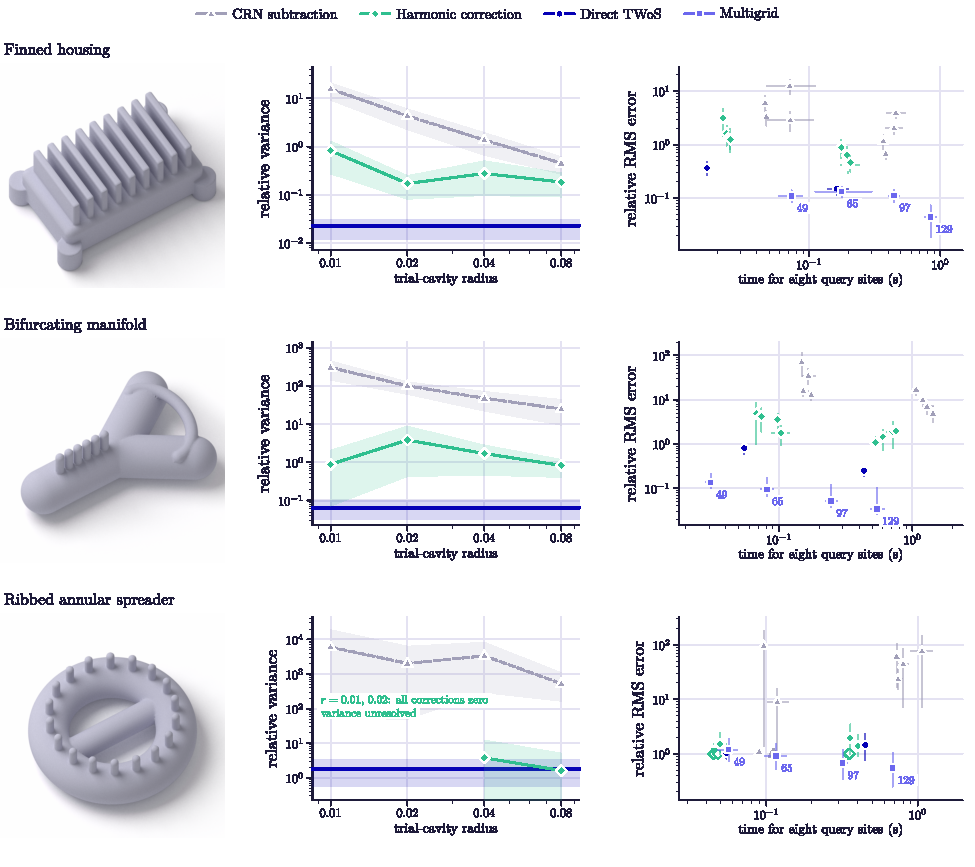
\includegraphics[width=\textwidth]{figures/submission-estimators.pdf}
 \caption{\textbf{Actual-geometry estimator comparisons.}
 Each row uses eight fixed, protected query sites on one mesh.
 The center plots normalize summed site variances by the squared norm of the
 high-budget reference and use 2,048 paths per site. Bands give pointwise 95\%
 bootstrap intervals from sixteen independent repeat vectors and sixteen
 independent reference batches. Direct TWoS has no trial-radius input;
 its horizontal band is repeated for comparison, not independently remeasured
 at every radius. Right: relative RMS error and wall time at both Monte Carlo
 budgets and all finite radii, with four deterministic grid resolutions labeled.
 Bars reflect repetition and reference-sampling uncertainty; deterministic
 grid error bars reflect only reference sampling, while their runtime bars
 use five repeated solves. Finite-radius, discretization,
 and termination biases are not enclosed. The reference is an independent,
 high-budget TWoS estimate, not exact ground truth. All-zero correction settings
 are marked unresolved and use open error--cost markers; their collapsed bootstrap intervals are suppressed.}
 \label{eg:submissionestimators}\label{fig:submissionestimators}
\end{figure}


\paragraph{Matched insertion and refinement.}
A finned housing, branching manifold, and ribbed annular spreader provide
different conduction paths. Each method inserts six disjoint radius-0.065
spheres from paired candidate pools, subject to identical source, sensor,
boundary, and pairwise clearance constraints. Every initialization then uses
the same specialized Differential WoS center-refinement component. TWoS,
multigrid at grid counts 49 and 65, and nearest-sensor placement receive eight
rounds; hottest-point and random starts receive sixteen. Five paired design
seeds are independently evaluated at saved checkpoints. This isolates the
initialization inside a shared optimizer; it does not reproduce the original
Differential WoS authors' complete application.

Mean sensor cooling after TWoS initialization and eight rounds is
$65.0\%$, $16.4\%$, and $11.4\%$ across the three objects. The primary
multigrid selector gives $65.1\%$, $16.3\%$, and $11.7\%$. Hottest-point
starts reach $42.7\%$, $0.14\%$, and $0.01\%$ despite twice as many rounds.
However, nearest-sensor placement reaches $63.6\%$, $17.3\%$, and $12.2\%$.
On the housing, complete mean times are 11.77 s for TWoS, 8.66 s for primary
multigrid, 7.99 s for coarse multigrid, and 7.08 s for nearest-sensor placement.
Thus the large benefit over hottest-point placement does not establish a
quality or speed advantage over all informed controls. The cutaways show
the stronger controls; the curves retain all six methods. Paired differences
and their pointwise intervals are reported in \cref{app:claimscope}; they do
not establish superiority over multigrid or equivalence to it.

\begin{figure}[tp]
 \centering
 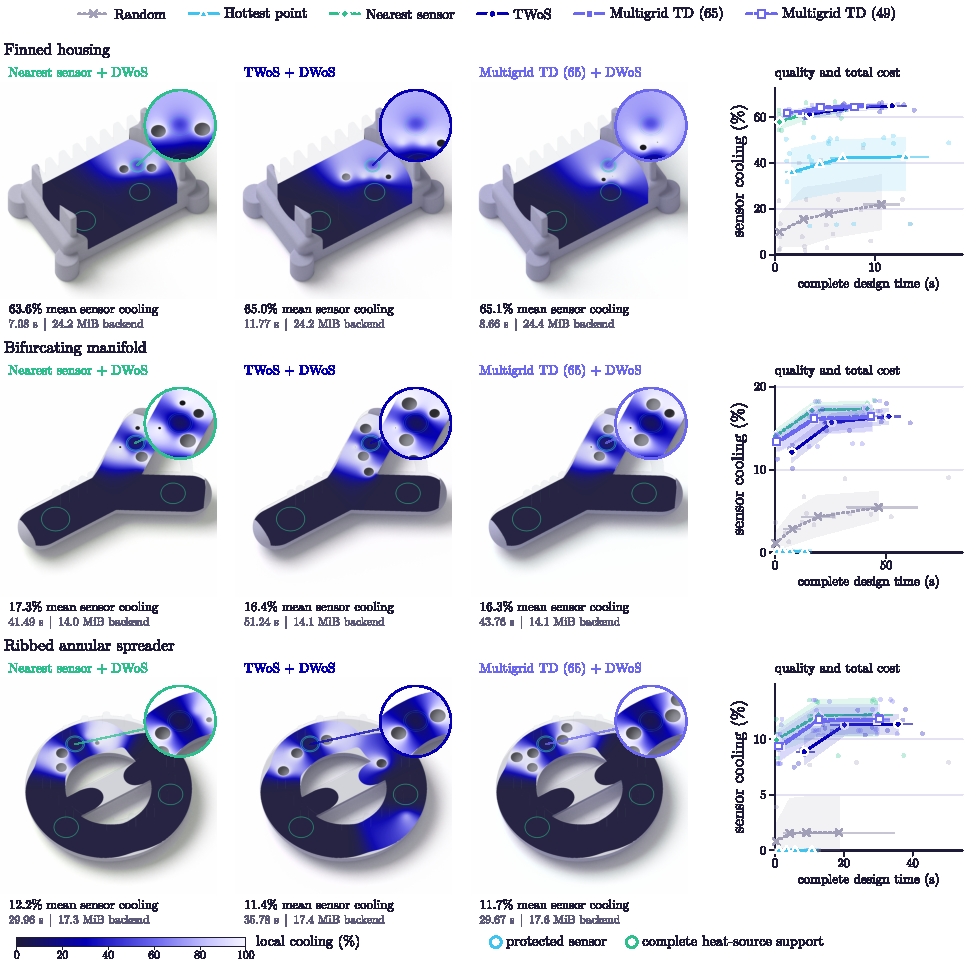
\includegraphics[width=\textwidth]{figures/submission-pipeline.pdf}
 \caption{\textbf{Insertion decisions affect the refined design.}
 Each row fixes the physical domain, protected sensor, heat input, cavity count,
 and exact removed volume. Views show the first predeclared seed after refinement;
 cyan and mint outlines mark the sensor and complete source supports. The
 section color shows local cooling relative to the unperforated temperature,
 from a common multigrid rendering field. It is not the objective's confidence
 interval. Labels and curves summarize five design seeds; faint dots show
 individual runs. Bands are pointwise 95\% bootstrap intervals for mean sensor
 cooling, jointly resampling seeds and independent evaluation blocks;
 horizontal bars resample complete runtime across seeds. Plot ranges adapt
 to each geometry; units and the local-cooling color scale are shared. They do not cover
 numerical bias. Hot and random receive up to sixteen refinement rounds;
 TWoS, both multigrid selectors, and nearest-sensor placement receive eight. Ghost shells show material
 removed only for display; some cavities lie outside the section. Independent evaluation, rendering, and mesh
 generation are excluded from design time.}
 \label{eg:submissionpipeline}\label{fig:submissionpipeline}
\end{figure}


\paragraph{Uncertainty and independent checks.}
The study contains 180 initial designs, 90 refinement runs, and 390 evaluated
states. Curves show means, individual runs, and pointwise 95\% bootstrap
intervals jointly resampling five paired design seeds and four shared
evaluation blocks. Tables additionally report the across-seed standard
deviation. These small-sample intervals exclude numerical bias. Every saved
state passes the geometric constraints, no recorded walk reaches its cap,
and the maximum multigrid relative residual is below $10^{-7}$.
Independent grid checks use 97 and 129 nodes on the longest axis; flagged
housing cases receive grids 193 and 257. The finest housing references still
differ from Monte Carlo reductions by up to 2.38 percentage points across
the checked first-seed designs, so small quality differences warrant caution.
The numerical audit does not certify reference accuracy.

\paragraph{Accessible channels at fixed material and heat input.}
Six open ball-union channels share a removed-volume target of 0.0168.
Every heat-source support is preserved, so the exact total heat input is
unchanged. Independent randomized volume audits deviate by at most 0.97\%
from the target; this is an observed audit error, not a certified bound.
TWoS gives mean regional cooling of $37.8\%$, $2.29\%$, and $1.75\%$,
versus $42.1\%$, $2.59\%$, and $1.93\%$ for primary multigrid.
Nearest-sensor placement gives $39.4\%$, $2.62\%$, and $2.02\%$.
This finite-channel heuristic is useful but does not dominate the informed
controls. Cutaways, volume audits, and full cost curves in the appendix report
the complete comparison.

\paragraph{Sparse queries at matched accuracy.}
Four meshes, two domain states, and nested batches of 8--512 fixed sites
compare TWoS against grids with 49--129 longest-axis nodes, using five paired
calibration seeds. Multigrid reuses solved fields; a stronger variant retains
outer masks and warm-starts after insertion. Compliance requires one solve.
Common mesh setup is measured separately. Our 20\% score-error target requires
an eligible upper bootstrap mean-error endpoint, MG193/MG257 refinement,
and independent Monte Carlo reference checks; it is not a continuum certificate.
A disclosed follow-up analytically integrates the prescribed sources using
classical Rao--Blackwellization (\cref{app:analytic-source}). This reduces
variance at fixed path count in ideal arithmetic, without removing termination
bias. \Cref{eg:matchedquery} compares objectives on the same Bunny; the full
protocol, ablations, reference gates, and stream correction are in
\cref{app:matchedaccuracy}.
All four calibration-selected apparent wins fail at least one confirmation
rule on 20 fresh paired seeds: three compliance cases exceed the accuracy
upper-endpoint threshold, while housing does not confirm a timing gain.
A separately declared follow-up fixes 256 walks at eight sites in both
compliance states, using 20 further fresh seeds. On the original Bunny,
TWoS takes 89.9 ms versus 113.9 ms for MG49: a $1.27\times$ ratio with
pointwise 95\% bootstrap interval $[1.05,1.50]$. Mean score error is
$9.0\%$ (upper endpoint $10.2\%$), versus $12.3\%$ for MG49.
After insertion, TWoS takes 83.1 ms versus 72.8 ms for warm-started MG;
the speed-ratio interval $[0.69,1.11]$ establishes no advantage.
This is a source-specific, eight-query result with geometry already loaded,
not a complete optimization speedup or universal state-of-the-art claim.

\begin{figure}[t]
\centering
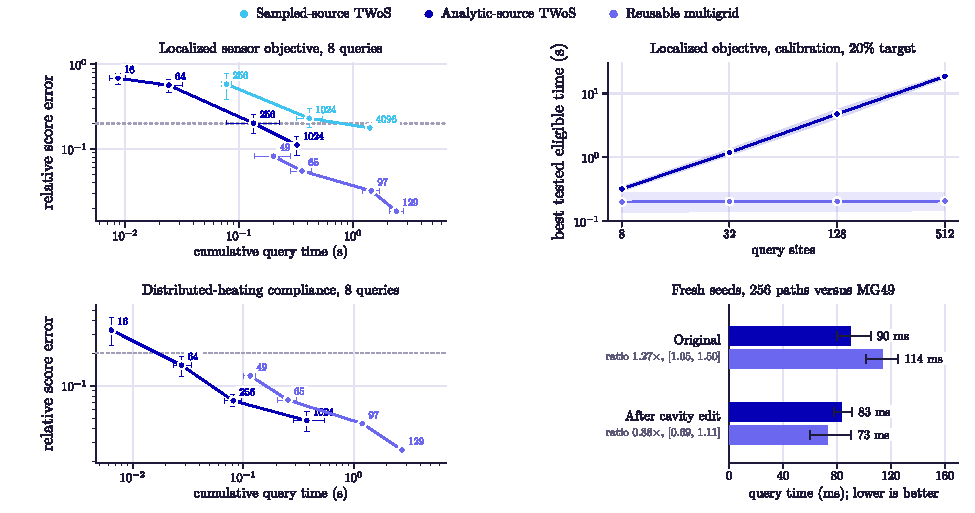
\includegraphics[width=\textwidth]{figures/matched-accuracy-bunny.pdf}
\caption{Same Bunny, different query workloads. Left: measured accuracy--cost
fronts at eight sites; labels give paths per site or longest-axis grid nodes.
Top right: fastest tested budgets passing the 20\% rule on five calibration seeds.
Bottom right: the separate fixed-budget confirmation on 20 fresh seeds; both
methods pass the 20\% error rule, but only the original-domain time ratio
confirms an advantage.
Bands and bars are pointwise 95\% bootstrap intervals; reference bias is excluded.
The analytic-source variant is restricted to the prescribed sources. Grid
curves use the faster eligible reuse implementation. Calibration fronts alone do not establish a speed claim.}
\label{eg:matchedquery}
\end{figure}

\paragraph{An exact finite-radius check.}
The uniformly heated ball with a concentric cooled cavity admits exact
states, compliance, and a positive certificate gap (\cref{app:exactcavity}).
Rational checks at 999 radii verify the algebra, not sampler coverage.

\paragraph{Validation has a separate cost.}
A guarded six-attempt compliance diagnostic on each of the Bunny and housing
uses a total failure budget of 0.01. All twelve targets pass, but validation
takes 150.39 s and 52.17 s versus 2.97 s and 0.53 s for scouting and rescoring.
Full bounds and independent checks are in the appendix. This additional
cost is excluded from ranking-only speed claims.
